
\section{Dark matter search}

\begin{figure}[htp]
    \centering
    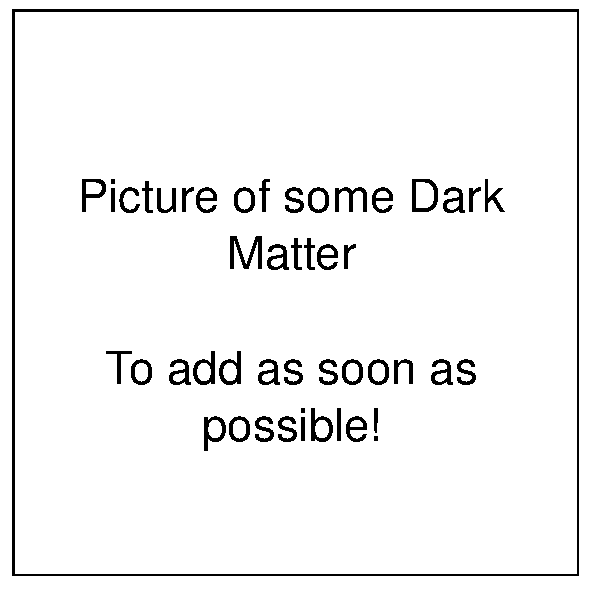
\includegraphics[width=0.3\textwidth]{Theory/figures/dark_matter_pic.pdf}
\end{figure}

The nature of dark matter (DM) is currently one of the most intriguing open questions in physics~\cite{Arbey2021}.
It's an active topic of research in astrophysics and cosmology, where it is implied as the accepted solutions for various phenomena, but is also of great interest for particle physicists, since it will inevitably go beyond the standard model.

Its existence, supported by theoretical models and experimental observations, it's widely accepted by the research community.\\
However, no direct proof has yet be found.

\subsection{Observational evidences}

There have been different evidences of the presence of DM.

\paragraph{Spiral galaxy rotational speed}

In spiral galaxies, the virial theorem dictates that the velocity of a star at distance $R$ from the center of the galaxy should follow~\cite{Belenchia2022}:
\begin{equation}
    v(R) = \sqrt{G\frac{M(R)}{R}}
\end{equation}
where $M(R)$ is the total mass contained a sphere with radius $R$.
Far from the center of the galaxy, where practically no mass is left and $M(R)$ is nearly constant, the velocity decreases as $v (R) \propto R^{-1/2}$.

However, experimental measurements of stars around spiral galaxies, performed with extremely precise Doppler shift measurements, shows a different picture.
In particular, it was observed that the velocity of stars becomes independent from the radius.
The phenomenon, visible for example in the \textit{flat rotation curves} of which \cref{fig:flat_rot_curves} are typical examples, can be explained with a halo of invisible mass of:
\begin{equation}
    M(R) = R\frac{v_0^2}{G}
\end{equation}

\begin{figure}
    \centering
    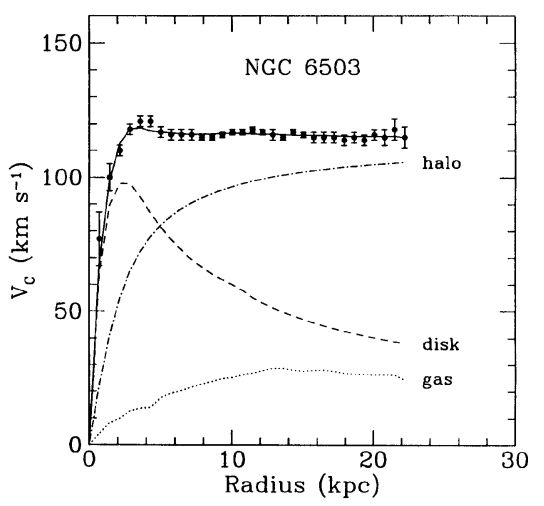
\includegraphics[width=9cm]{Theory/figures/flat_rot_curves.jpg}
    \caption[Flat rotation curves]{Galactic rotation curve for NGC 6503 showing disk and gas contribution plus the dark matter halo contribution needed to match the data. Credits to \cite{fig_rot}}
    \label{fig:flat_rot_curves}
\end{figure}

Since this mass, that seems to represent up to 80-90\% of the total mass of galaxies, appears to not interact in any way except by gravitational force, we identify it and call it as Dark Matter (DM).

\paragraph{Galaxy clusters dynamic}

A Galaxy cluster is a massive object composed of hundreds or thousands of galaxies bound together. 
In the intergalactic medium, among galaxies, it contains large quantity of gases that reach high velocities and can emit x-rays via bremsstrahlung.
This effect can be used as a way of measuring the intensity of the gravitational force and, therefore, the distribution of masses in the cluster.
The idea is that photons emitted from the center of the cluster should lose more energy than photons emitted from the edge, because of a stronger gravity.
This effect, known as \textit{gravitational redshift}, showed that a large portion of mass was not visible and distributed all around the cluster.

This method leads to results with high uncertainties, so it has been superseded by gravitational lensing techniques.

\paragraph{Gravitational lensing}

The observation of distant galaxies and galaxy clusters is usually affected by the gravitational lensing phenomenon depicted in \cref{fig:grav_lense}.
Namely, the light does not follow a straight line, being distorted by any mass between source and observer (the earth) forming the so-called \textit{Einstein circle}.

\begin{figure}
    \centering
    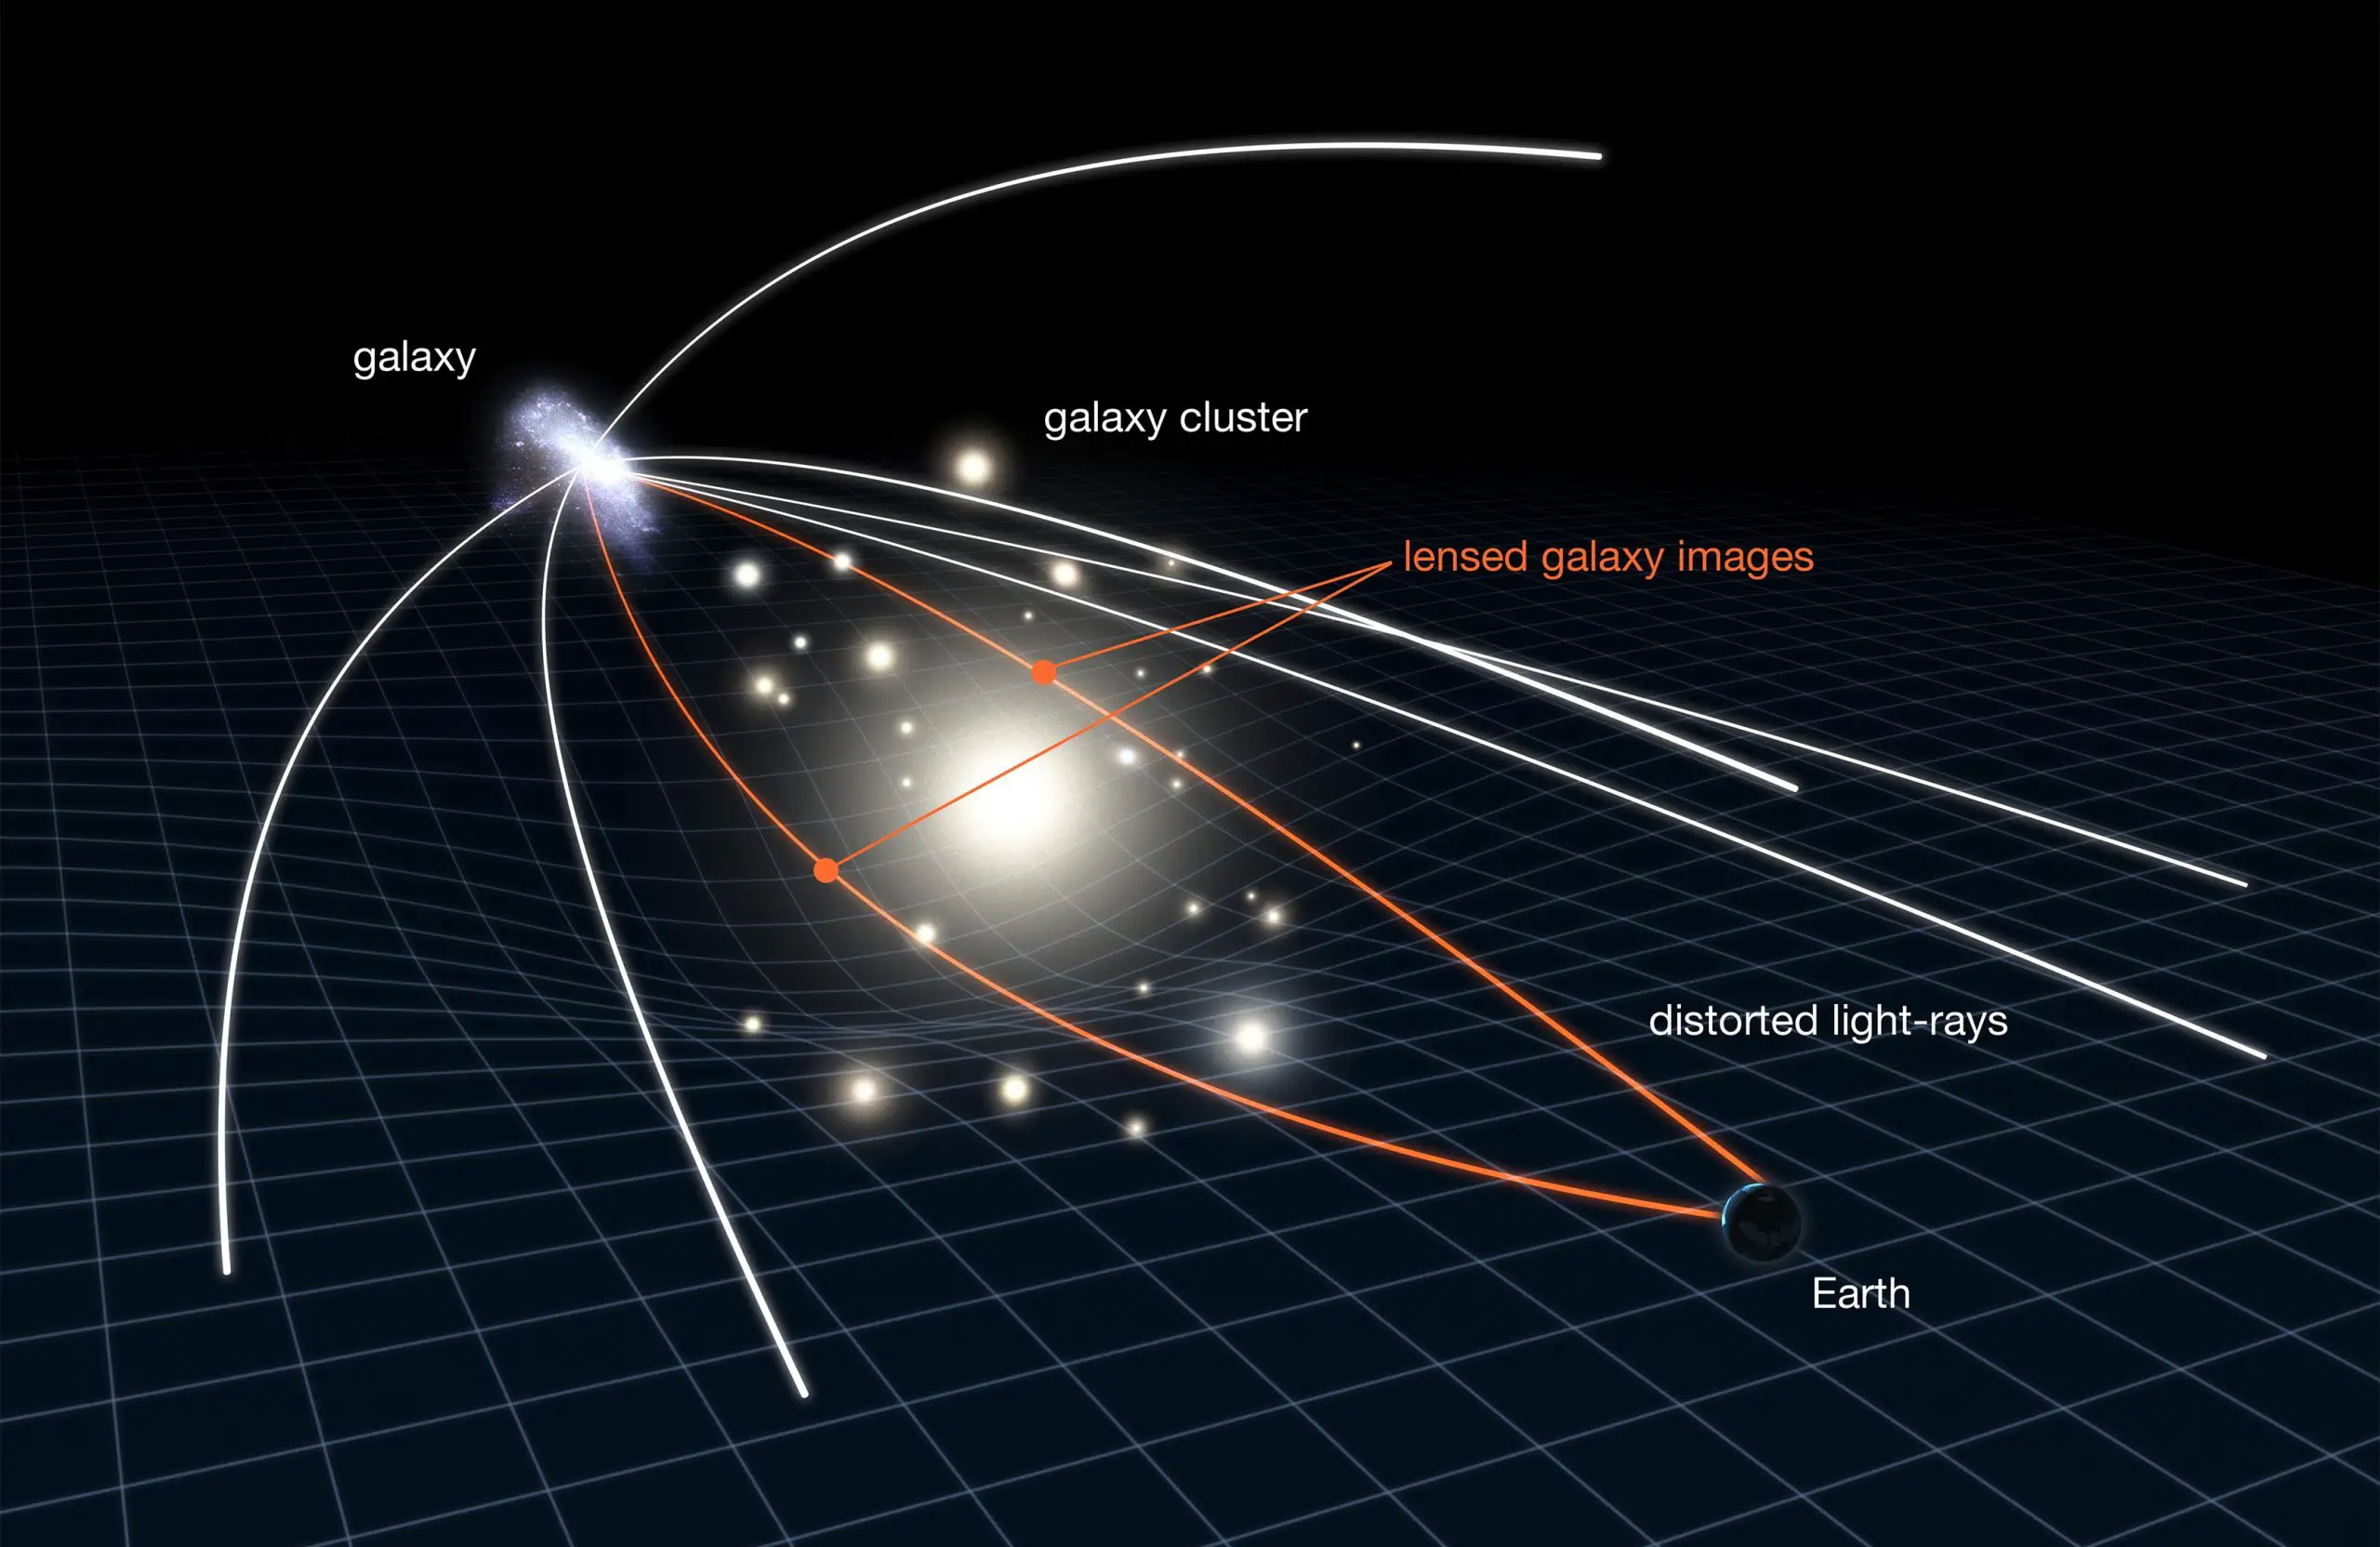
\includegraphics[width=\textwidth]{Theory/figures/gravitational_lense.png}
    \caption[Graphical depiction of gravitational lensing]{This illustration depicts the gravitational lensing phenomenon. The scale has been greatly exaggerated in this diagram. Credits to \cite{fig_lensing}}
    \label{fig:grav_lense}
\end{figure}

The radius of an Einstein circle is related to the mass which causes the light deflection following:
\begin{equation}
    \theta_E = \sqrt{\frac{4GM}{c^2}\frac{(D_S-D_L)}{D_S D_L}}
\end{equation}
with $\theta_E$ being the angular radius, $M$ the mass of the lens (in between) , $D_L$ the distance to the lens and $D_S$ the distance to the source.
This technique to weigh galaxies (and other astrophysical structures) has been used with success for many years.
Numerous studies, however, consistently reported a much larger mass measured than seen.
Again, this is explainable with presence of DM.



\paragraph{Cosmology}

The currently most widely accepted cosmological theory requires dark matter to explain the formation of structures in the early universe.

In particular, in the early universe, the energy distribution (so the mass distribution) was more or less uniform.
Two opposite processes were involved in the generation of structures: gravitational forces that were favouring structures and the expansion of the universe itself, that was "countering" structures.

In this situation, it is possible to differentiate the role of baryonic and non baryonic matter that is collisionless.
Various simulations, and in particular the Millennium Simulation~\cite{Springel2005}, were able to simulate all the early stages of the universe, with the requirement of dark matter and dark energy. 
Without DM, the current model was not able to explain nor the structures formation nor the CMB spectrum.

The current best theory, the $\Lambda$CDM (Lambda cold dark matter) shows a remarkable agreement with all the observations from disparate scales as shown in \cref{fig:convergence_dm}.

\begin{figure}
    \centering
    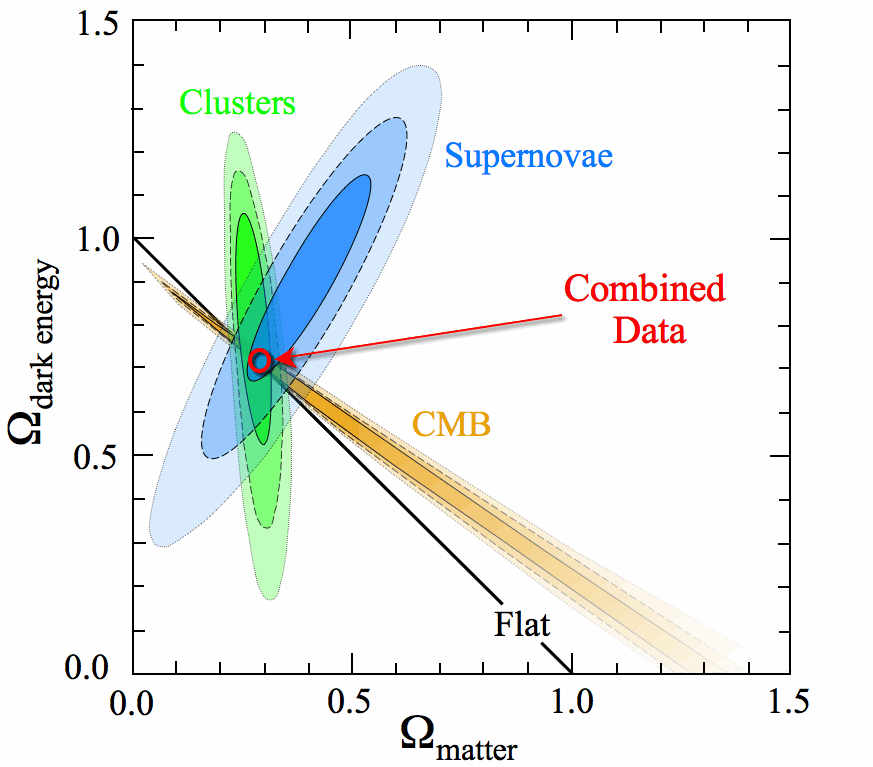
\includegraphics[width=0.6\textwidth]{Theory/figures/dark_energy_concordance.png}
    \caption[Dark Matter quantity expected from observations and theory]{Convergence of the experimental observations and of the $\Lambda$CDM model. Leading to a a percentage of $95$\% of non-baryonic energy. Credits to \cite{Einasto2009}}
    \label{fig:convergence_dm}
\end{figure}

\subsection{DM candidates}

Now that we saw the many evidences supporting the existence of dark matter, the challenge becomes to determine its nature.

We are looking for a particle (or, for what we know, a set of particles) that is stable over billions of years, collisionless, non-baryonic and interacting mostly gravitationally.

Within the Standard Model (SM), the only neutral non-baryonic particles are the neutrinos that are, however, very light particles.
This leads neutrinos to be generally relativistic, constituting an example of fast or "hot" DM.
The CMB spectrum, however, cannot be properly explained with only "hot" (relativistic) DM and rather requires the presence of a large quantity of "cold" (non relativistic) particles.
Therefore the neutrinos can eventually explain just a minimal portion of the hidden mass.
We need to find new particles, beyond SM.

Tens of candidates, of which the main ones are shown in \cref{fig:dm_candidates}, have been proposed over the years, but none has been yet successfully discovered. Indeed this is also referred to as the "dark matter candidates zoo", because of the large and never ending number of proposed new  particles.\\
Since this thesis is not directly focused on DM, we will briefly mention the two main candidates: WIMPs (weakly interacting massive particles) and axions.

\begin{figure}[ht]
    \centering
    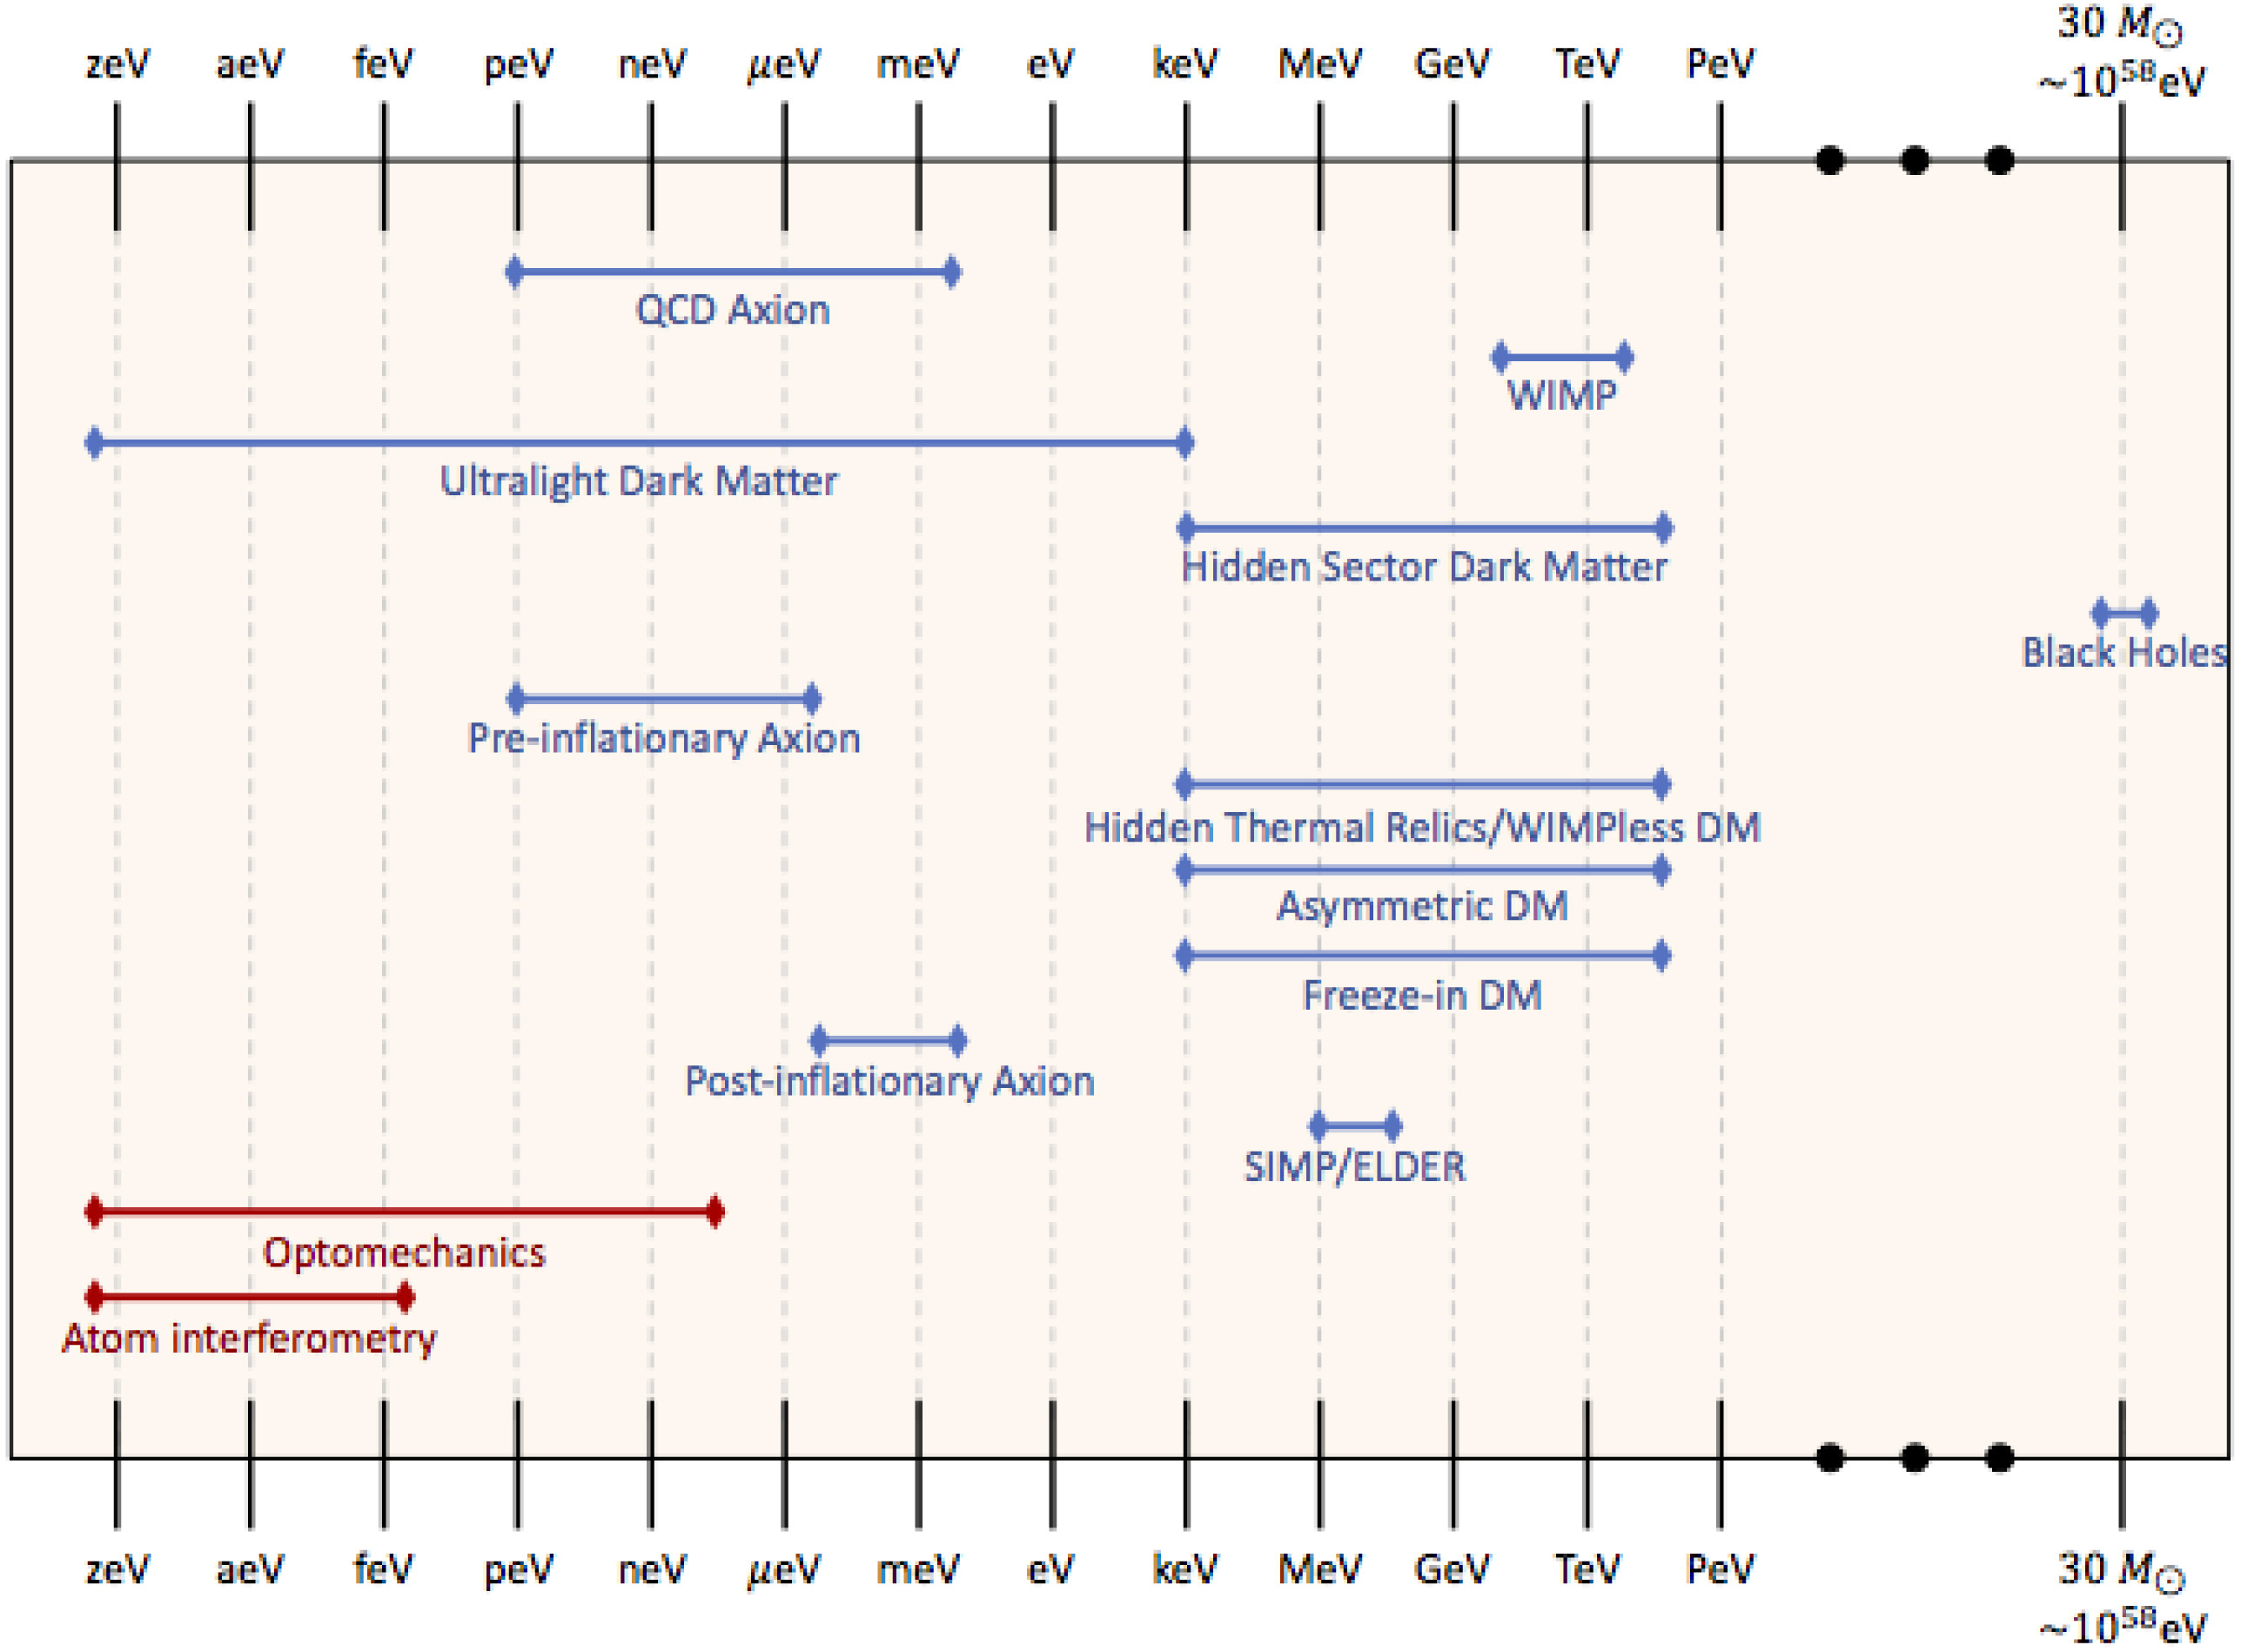
\includegraphics[width=\textwidth]{Theory/figures/candidates_dm.jpg}
    \caption[Dark Matter candidates]{DM candidates, in respect to the possible masses. Credits to \cite{Belenchia2022}}
    \label{fig:dm_candidates}
\end{figure}


\paragraph{WIMPs} were, until very recently, the most prominent DM candidate. With the name of WIMPs, various particles were described. They were supposed to have been produced thermally in the early universe (as the SM particles) with a mass of $\approx 100$ GeV. The introduction of WIMPs was often referred to as the "WIMPs miracle" since these particles are "automatically" introduced with a minimal extension of the SM to a super-symmetric theory. Moreover, WIMPs should have been detectable both indirectly, looking at annihilation products, and directly in collision experiments. No experiment\footnote{With the notable exception of the non-reproducible results of DAMA~\cite{Petriello2008}.} has ever found direct evidence and, lately, the hype for super-symmetric theories has also been decreasing, since no evidence has yet to be found ad LHC and other colliders (although it was indeed expected).

\paragraph{Dark Photons}~\cite{Caputo2021} introduce an intriguing dimension to the realm of dark matter, akin to WIMPs and axions. These hypothetical particles, often associated with hidden or "dark" forces that operate outside the framework of the Standard Model of particle physics, are captivating for their unique characteristics. Dark photons are postulated as mediators of a novel force, commonly termed the "dark force," which interacts exceptionally weakly with ordinary matter. Just as with their counterparts, dark photons may trace their origins back to the early universe, potentially emerging through mechanisms reminiscent of WIMPs.
Dark Photons still are a viable candidate, but require a large theoretical extension of the Standard Model and, being also particularly difficult to detect, are often discarded in comparison to other candidates. 

\paragraph{Axions} The original axion model is related to the strong violation of the charge conjugation (C) and parity (P) symmetries (CP-violation). The QCD Lagrangian can be written as 
\begin{equation}
    \mathcal L _{QCD} = \mathcal L _{QCD, perturbative} + \Bar{\theta} \frac{g^2}{32 \pi^2} G^a_{\mu \nu} \Bar{G}^a_{\mu \nu}
\end{equation}
where $G^a_{\mu \nu}$ is the gluon tensor, $\Bar{G}^a_{\mu \nu}$ its dual and $\Bar{\theta}$ a constant. The first term is the standard perturbative Lagrangian and the second one is an effective term coming from the topological properties of non-Abelian gauge theories and from the diagonalization of the quark mass matrix.
The problem with this term is that it violates the P and CP symmetries and measurements on the neutron electric dipole moment reveal no violation of those symmetries for the strong-force. 
A solution for this missing violation was proposed by Peccei and Quinn, in which the constant is substitute with a dynamical term coming from a new chiral global symmetry $U(1)$. This new symmetry spontaneously break and gives rise to a new scalar boson, called "axion". The symmetry also generates a new term in the Lagrangian, that removes the violation. From theory we have that:
\begin{equation}
    m \approx \frac{\Lambda^2_{QCD}}{f_a}
\end{equation}
where $m$ is the expected mass of the new particle (ranging from $\mu$eV and eV), $\Lambda_{QCD}\approx 200$ MeV and $f_a$ is a constant with the dimension of an energy, of the order of the symmetry breaking scale.

Axions are an interesting candidate for these reasons: they were not introduced for DM and solve two huge problems of modern physics. They could indeed explain the missing mass of the universe, while at the same time solving the strong CP problem.

